\section{Discussion}

\subsection{Task 1: \cartpole with vanilla DQN}

\subsubsection{Training Commands}

For the task 1, which required to use the vanilla DQN algorithm, I used the following command to train the agent:

\begin{minted}{bash}
python3 trainer.py --env cartpole --exp report --vanilla --epsilon-decay 0.99
\end{minted}

The command specifies the environment as \cartpole, the experiment name as \texttt{report}, and the epsilon decay rate as 0.99.
The \texttt{----vanilla} flag indicates that the agent should use the vanilla DQN algorithm without any modifications. Unlike Double DQN (DDQN), vanilla DQN uses the same network for both action selection and value estimation, which can lead to overestimation of Q-values. DDQN mitigates this issue by using the target network for value estimation while using the main network for action selection.
The \texttt{----epsilon-decay} flag specifies the decay rate for the epsilon value, which controls the exploration-exploitation trade-off during training.
The other hyperparameters are set to their default values.

The hyperparameters values are as follows:
\begin{itemize}
    \item \textbf{Batch size}: $32$
    \item \textbf{Discount factor}: $0.99$
    \item \textbf{Learning rate}: $0.0001$
    \item \textbf{Memory size}: $100,000$
    \item \textbf{Epsilon start}: $1$
    \item \textbf{Epsilon decay}: $0.99$
    \item \textbf{Epsilon min}: $0.015$
    \item \textbf{PER alpha}: $0$
    \item \textbf{PER beta}: $1$
    \item \textbf{N Steps}: $1$
    \item \textbf{Update Period}: $1$
    \item \textbf{Number of episodes}: $500$
    \item \textbf{Seed}: $42$
    \item \textbf{Evaluation episodes}: $10$
\end{itemize}

The training process consists of $500$ episodes, and the evaluation reward is calculated as the average reward over $10$ evaluation episodes.
The training process is performed using the \texttt{Trainer} class, which handles the training loop and updates the model.

\subsubsection{Training Curves}

The training curves for the task 1 are shown in Figure \ref{fig:cartpole-training-curve}.

\begin{figure}[H]
    \centering
    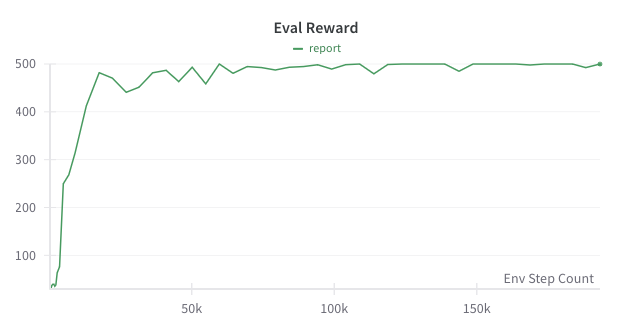
\includegraphics[width=0.8\textwidth]{figures/task1.png}
    \caption{Training curves for the \cartpole environment.}
    \label{fig:cartpole-training-curve}
\end{figure}

\subsubsection{Testing Commands}

We can test the trained agent using the following command:
\begin{minted}{bash}
python3 tester.py --env cartpole --exp report --model ./results/cartpole/report/best_model.pt --episodes 30
\end{minted}

This can achieve the score over than $480$ in 30 consecutive episodes.

\subsection{Task 2: \pong with vanilla DQN}

\subsubsection{Training Commands}

For the task 2, which required to use the vanilla DQN algorithm, I used the following command to train the agent:

\begin{minted}{bash}
python3 trainer.py --env pong --exp report --vanilla --episodes 2500 --eval-episodes 2
\end{minted}

The command specifies the environment as \pong, the experiment name as \texttt{report}, and the \texttt{----vanilla} flag indicates that the agent should use the vanilla DQN algorithm without any modifications.
Unlike Double DQN (DDQN), vanilla DQN uses the same network for both action selection and value estimation, which can lead to overestimation of Q-values.
DDQN mitigates this issue by using the target network for value estimation while using the main network for action selection.
The \texttt{----episodes} flag specifies the maximum number of episodes for training, which is set to $2500$ in this case.
The \texttt{----eval-episodes} flag specifies the number of evaluation episodes, which is set to $2$ in this case.
The other hyperparameters are set to their default values.

The hyperparameters values are as follows:
\begin{itemize}
    \item \textbf{Batch size}: $32$
    \item \textbf{Discount factor}: $0.99$
    \item \textbf{Learning rate}: $0.000025$
    \item \textbf{Memory size}: $100,000$
    \item \textbf{Epsilon start}: $1$
    \item \textbf{Epsilon decay}: $0.99999$
    \item \textbf{Epsilon min}: $0.005$
    \item \textbf{PER alpha}: $0$
    \item \textbf{PER beta}: $1$
    \item \textbf{N Steps}: $1$
    \item \textbf{Update Period}: $1$
    \item \textbf{Number of episodes}: $500$
    \item \textbf{Seed}: $42$
    \item \textbf{Evaluation episodes}: $2$
\end{itemize}

\subsubsection{Training Curves}

The training curves for the task 2 are shown in Figure \ref{fig:pong-vanilla-training-curve}.

\begin{figure}[H]
    \centering
    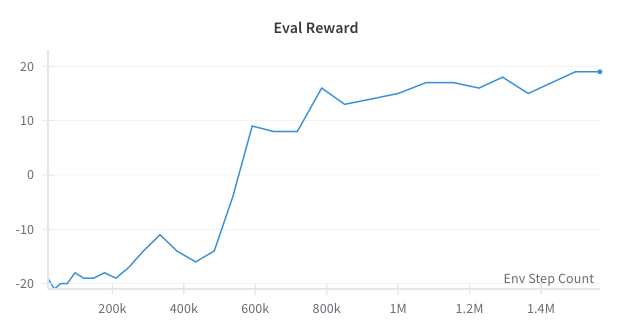
\includegraphics[width=0.8\textwidth]{figures/task2.png}
    \caption{Training curves for the \pong environment.}
    \label{fig:pong-vanilla-training-curve}
\end{figure}

We can see that the agent can achieve the score of $19$ in some of the evaluation episodes.

\subsubsection{Testing Commands}

We can test the trained agent using the following command:
\begin{minted}{bash}
python3 tester.py --env pong --exp report --model ./results/pong/report/best_model.pt --episodes 20
\end{minted}
This can achieve the score of $19.45$ in 20 consecutive episodes.

\subsection{Task 3: \pong with DQN Variants}

\subsubsection{Training Commands}

For the task 3, which required to use the DQN variants.

However, I use the vanilla DQN algorithm for the \pong environment and \textbf{it can \textcolor{red}{achieve the score of $21$} (evaluated in 30 consecutive episodes) in about \textcolor{red}{$140k$ environment steps}}.

The training commands are as follows:

\begin{minted}{bash}
python3 trainer.py --env pong --exp task3 --vanilla --update-period 1 --n-step 1
\end{minted}

The command specifies the environment as \pong, the experiment name as \texttt{task3}, and the \texttt{----vanilla} flag indicates that the agent should use the vanilla DQN algorithm without any modifications.

The other hyperparameters are set to their default values.
The hyperparameters values are as follows:
\begin{itemize}
    \item \textbf{Batch size}: $32$
    \item \textbf{Discount factor}: $0.99$
    \item \textbf{Learning rate}: $0.0001$
    \item \textbf{Memory size}: $100,000$
    \item \textbf{Epsilon start}: $1$
    \item \textbf{Epsilon decay}: $0.99999$
    \item \textbf{Epsilon min}: $0.005$
    \item \textbf{PER alpha}: $0$
    \item \textbf{PER beta}: $1$
    \item \textbf{N Steps}: $1$
    \item \textbf{Update Period}: $1$
    \item \textbf{Number of episodes}: $500$
    \item \textbf{Seed}: $42$
    \item \textbf{Evaluation episodes}: $10$
\end{itemize}

\subsubsection{Training Curves}

The training curves for the task 3 are shown in Figure \ref{fig:pong-task3-training-curve}.
\begin{figure}[H]
    \centering
    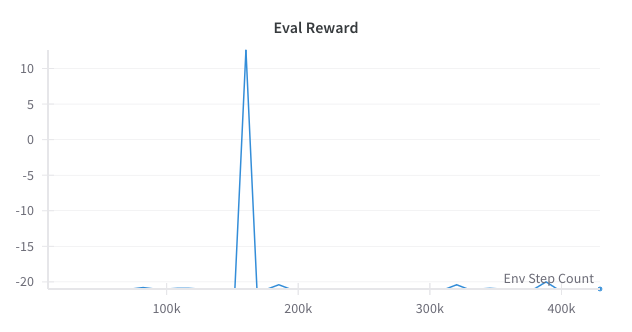
\includegraphics[width=0.8\textwidth]{figures/task3.png}
    \caption{Training curves for the \pong environment.}
    \label{fig:pong-task3-training-curve}
\end{figure}

We can see that the evaulation result shows that the agent can not achieve well performance in the \pong environment. It always get the score of $-21$ except a special snapshot that the agent can get the score over than $10$.
By the way, this evaluation score during the training process is the average score of 10 episodes.

After inspecting the special snapshot, I found that the agent can get the score of $21$ in some episodes by moving to a specific position and hitting the ball at the right time without moving the paddle again.
However, in the other episodes, the agent can not hit any ball and the score is $-21$.

\subsubsection{Testing Commands}

Therefore, during the testing process, if we use this snapshot to test the agent in the \pong environment, the agent can get the score of $21$ in 30 consecutive episodes by the following testing command:
\begin{minted}{bash}
python3 tester.py --env pong --exp task3 --model ./results/pong/task3/best_model.pt --seed 92439410 --episodes 30
\end{minted}

The command specifies the environment as \pong, the experiment name as \texttt{task3}, and the \texttt{----model} flag indicates that the agent should use the model saved in the \texttt{best\_model.pt} file, you should change the path to your own path.
The \texttt{----seed} flag specifies the first random seed for the environment, and the following seed for the environment will be $seed + \text{episode\_number}$. That is to say, the first episode will use the seed $92439410$, the second episode will use the seed $92439411$, and so on.
The \texttt{----episodes} flag specifies the number of evaluation episodes, which is set to $30$ in this case.

\subsection{Analyze each Technique}

The following sections outline the key techniques employed in the DQN algorithm and their impact on the training process.
Due to the extensive number of experiments conducted, including numerous subtle variations in hyperparameters, this report focuses on describing the techniques and analyzing their effects rather than presenting all training curves.
For further details or to reproduce the results, please refer to the implementation in the \texttt{trainer.py} and \texttt{dqn.py} files.

\subsubsection{Double DQN}

Vanilla DQN uses a single target network to estimate the Q-value of the action it also selected, which tends to overestimate action values because both selection and evaluation share the same (noisy) numbers.
Double DQN (DDQN) keeps the overall architecture and loss function the same but splits those two roles: the online network picks the action \(a^{\*}=\arg\max_a Q_{\text{online}}(s',a)\), while the target network supplies its value \(Q_{\text{target}}(s',a^{\*})\) for the TD target.
By decoupling selection from evaluation, DDQN dramatically reduces this positive bias, yielding more accurate value estimates, stabler learning curves, and usually better final performance—especially in environments with many actions or large reward variance—without adding extra networks or hyper-parameters beyond the standard target-network update already present in DQN.

\subsection{Prioritized Experience Replay}

Prioritized Experience Replay (PER) replaces the uniform-random sampling used in vanilla DQN's replay buffer with a probability \(P_i \propto |\delta_i|^{\alpha}\), where \(\delta_i\) is the transition's latest TD-error and \(\alpha\in[0,1]\) controls how aggressively "surprising" experiences are favored.
Transitions that the network currently mis-predicts (large \(|\delta|\)) are therefore replayed more often, accelerating the correction of large errors and speeding convergence.
% Because this biased sampling breaks the i.i.d. assumption, PER attaches an importance-sampling weight \(w_i=(1/N\;·\;1/P_i)^{\beta}\) (with annealed \(\beta\in[0,1]\)) to each gradient to recover an unbiased estimate of the expected update.
Because this biased sampling breaks the i.i.d. assumption, PER attaches an importance-sampling weight $w_i = (\frac{1}{N}\frac{1}{P_i})^{\beta}$ (with annealed \(\beta\in[0,1]\)) to each gradient to recover an unbiased estimate of the expected update.
In practice, PER improves sample efficiency and final scores on many Atari and continuous-control tasks, costs only an extra log-time lookup via a SumTree or segment tree, and stacks well with other improvements like Double DQN or dueling networks—but it introduces two extra hyper-parameters (\(\alpha, \beta\)) and can over-focus on a small subset of transitions if \(\alpha\) is set too high.


\subsection{Multi-Step Learning}

Multi-step (n-step) learning replaces DQN's single-step TD target with an \(n\)-step return that rolls rewards forward for \(n\) steps before bootstrapping:
\[
    G^{(n)}_t = r_t + \gamma r_{t+1} + \dots + \gamma^{n-1} r_{t+n-1} + \gamma^{n} \max_{a'}Q_{\text{target}}(s_{t+n},a').
\]
This amplifies the learning signal by injecting several real rewards before any bootstrapping noise, letting the agent propagate credit faster through time and making early training less sensitive to inaccurate value estimates.
Because the return mixes Monte-Carlo (more accurate but high-variance) and TD (more biased but low-variance) signals, \(n\) controls a bias-variance trade-off: \(n=1\) reduces to vanilla DQN, \(n\to\infty\) becomes a full Monte-Carlo target, and typical values \(n\in[3,10]\) give the best of both worlds.
Multi-step targets are cheap to compute in a replay buffer (store cumulative discounted reward and terminal flag) and combine smoothly with other upgrades such as Double DQN and PER, often yielding faster convergence and higher final scores—especially in sparse-reward or long-horizon tasks—without adding new networks or extra hyper-parameters beyond the choice of \(n\).


\subsection{Additional Training Tricks}

\subsubsection{Multiple Evaluation Episodes}

I found that the evaluation process is stochastic and the evaluation score is not stable during the training process.
This means that the evaluation score can be affected by the random seed used in the environment and will cause the evaluation score to be unexpectly high or low.
This will cause the stored best model to be not the best model in the training process.
Therefore, I used multiple evaluation episodes to calculate the average evaluation score during the training process.
This can help to reduce the variance of the evaluation score and make the evaluation score more stable.
This can be achieved by using the \texttt{--eval-episodes} flag in the training command.
The \texttt{--eval-episodes} flag specifies the number of evaluation episodes, which is set to $10$ by default.

\subsubsection{Learning Rate Scheduler}

I found that the learning rate is a very important hyper-parameter in the training process.
The learning rate controls the step size of the gradient descent algorithm and can affect the convergence speed and stability of the training process.
From my experiments, I found that if the learning rate is too high, the training process will stuck at a suboptimal solution and the evaluation score will not improve no matter how many episodes are trained.
On the other hand, if the learning rate is too low, the training process will be very slow and the evaluation score, but the evaluation score will keeps improving.
Therefore, I used a learning rate scheduler to reduce the learning rate during the training process, which can help to improve the convergence speed and stability of the training process.
